\section{DESIGN DE INTERFACE E TELAS DO SISTEMA WeFIND}

O design de interface de um aplicativo móvel voltado à utilidade pública é fundamental para que ele funcione bem na prática. Essa importância cresce ainda mais em momentos de emergência e estresse, como na perda de um animal de estimação, quando o tutor se encontra abalado emocionalmente e precisa agir com rapidez. Como destacam Rogers, Sharp e Preece (2023), o projeto de interação humano-computador (IHC) deve ter como foco diminuir a carga cognitiva do usuário. Isso significa criar telas diretas, organizadas e com navegação intuitiva, permitindo que a pessoa encontre o que precisa e execute ações importantes sem se sentir confusa ou perdida no aplicativo.

No WeFIND, a construção das telas foi orientada por critérios de usabilidade, com destaque para as dez heurísticas de Nielsen (1994) adaptadas ao contexto dos smartphones e para as orientações da norma ABNT NBR ISO 9241-11 (ABNT, 2021). A norma define usabilidade a partir de eficácia, eficiência e satisfação. Esses princípios orientaram a organização dos fluxos de navegação, cadastro e registro de avistamentos; a verificação da experiência dos usuários será realizada na avaliação planejada.

Outro cuidado central foi a acessibilidade digital, orientada pelas diretrizes internacionais da \textit{Web Content Accessibility Guidelines} (WCAG 2.1), no nível recomendado AA (W3C, 2023). No WeFIND, essas diretrizes serviram como referência para decisões de contraste, legibilidade e dimensões das áreas de toque, especialmente considerando o uso do smartphone em ambientes externos. A conformidade efetiva deverá ser verificada por inspeção e testes específicos.

Dessa maneira, o projeto visual buscou harmonizar clareza de informações, ergonomia e acolhimento. As subseções a seguir apresentam as escolhas tipográficas, a identidade visual, a paleta de cores e os principais fluxos de telas da plataforma WeFIND.


\subsection{Tipografia e Hierarquia Visual}

A definição tipográfica constitui a base fundamental do design de interface do WeFIND, visto que a legibilidade rápida de textos de alerta, características físicas dos animais e endereços é indispensável em momentos de urgência. A Figura~\ref{fig:tipografia} apresenta a família tipográfica adotada na aplicação.

\begin{figure}[H]
    \centering
    \caption{Família Tipográfica Roboto Adotada no WeFIND}
    \label{fig:tipografia}
    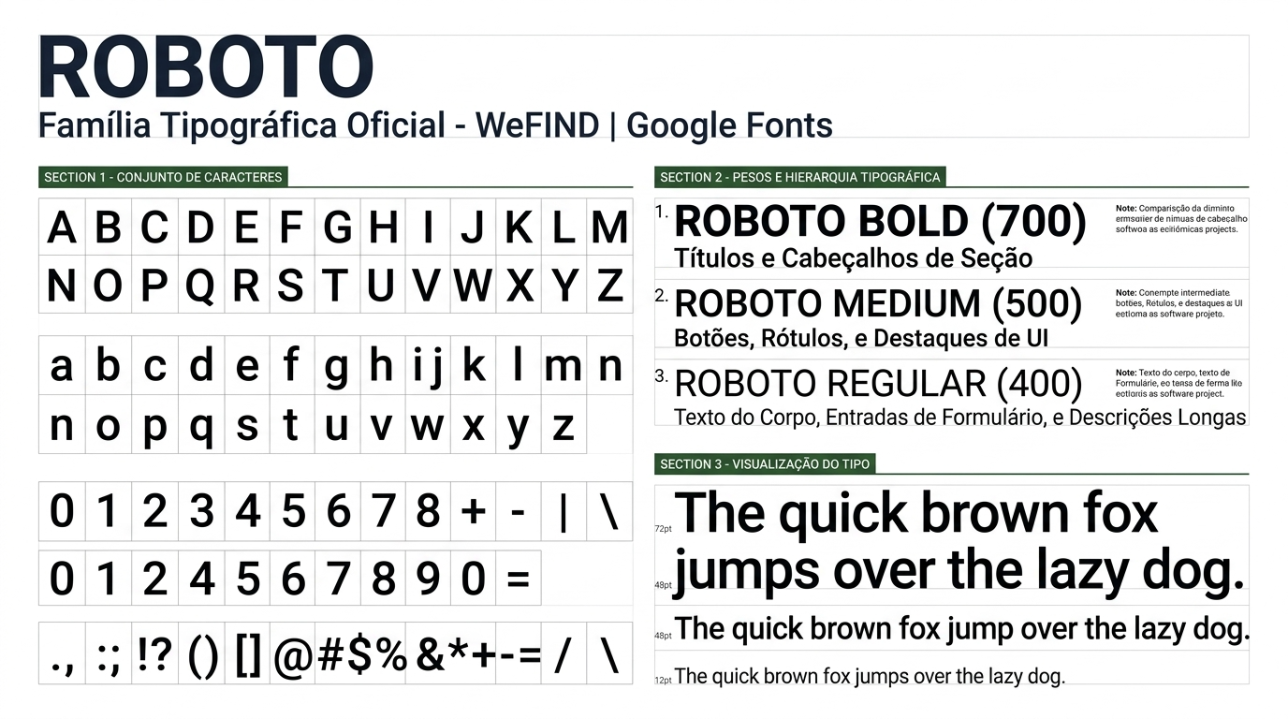
\includegraphics[width=0.85\textwidth]{imagens/03_arquitetura_design/figura15_tipografia_roboto.png}
    \fonte{Google Fonts (2024)}
\end{figure}

Adotou-se a família tipográfica sem serifa Roboto (GOOGLE FONTS, 2024), consagrada no ecossistema móvel por suas proporções geométricas equilibradas, ampla abertura de glifos e excelente legibilidade em telas com variadas densidades de pixels. A hierarquia visual do WeFIND fundamenta-se no uso combinado de três pesos da fonte, em que o peso em negrito (\textit{bold}) é aplicado prioritariamente em títulos de tela, nomes de animais, valores de recompensa e marcadores de estado para conduzir a atenção primária do usuário. Por sua vez, o peso médio (\textit{medium}) é empregado em rótulos de botões de ação, elementos da barra de navegação inferior e etiquetas de atributos físicos como espécie, raça e porte, ao passo que o peso regular é destinado aos corpos de texto descritivos, relatos de avistamentos e orientações contextuais de preenchimento. O  espaçamento entrelinhas e as margens de toque mínimas de 48 por 48 pixels para áreas clicáveis foram calibrados em estrita conformidade com as diretrizes de ergonomia móvel, assegurando conforto visual e operabilidade eficiente com apenas uma mão.


\subsection{Identidade Visual e Conceito do Aplicativo}

A identidade visual do WeFIND foi projetada para transmitir sentimentos de solidariedade comunitária, segurança, afeto e esperança. A própria denominação da plataforma une o pronome coletivo em língua inglesa ``We'' (Nós) ao verbo ``Find'' (Encontrar), expressando a premissa de que o resgate de um animal de estimação não é um drama individual, mas uma missão compartilhada entre toda a vizinhança.

Para fortalecer esse elo comunitário, a identidade visual do WeFIND priorizou uma atmosfera que transmite afeto, acolhimento e esperança. O objetivo foi criar uma marca que despertasse empatia imediata e incentivasse a colaboração espontânea da vizinhança, mostrando que a união de pessoas apoiada pela tecnologia pode ser uma aliada calorosa e confiável em momentos delicados.

A inclusão conjunta do cão e do gato no símbolo gráfico reflete a realidade do convívio familiar brasileiro. Embora muitas campanhas de proteção animal concentrem-se historicamente apenas em cães, a perda e o abandono de felinos representam ocorrências igualmente frequentes e dolorosas no ambiente urbano. Ao reunir as duas espécies em harmonia visual, a marca consolida desde o primeiro contato que a plataforma foi concebida para acolher tutores de ambos os animais com o mesmo nível de atenção.

Para a concepção do ícone oficial, utilizou-se a ferramenta de inteligência artificial generativa Flow Labs (FLOW LABS, 2026), integrada ao processo de design no Figma. O uso de inteligência artificial generativa permitiu explorar variadas composições visuais em poucos minutos, auxiliando na definição de um conceito moderno e equilibrado.

Os critérios solicitados incluíram estilo minimalista e plano (\textit{flat design}), adequado para ícones em telas móveis de diversos tamanhos. Buscou-se a integração harmoniosa de silhuetas representativas do universo doméstico: o perfil amigável de um cão e de um gato, simbolizando as principais espécies acolhidas pelas famílias. No centro, posicionou-se o marcador de mapa, representando a busca ativa por satélite, com as cores terracota e verde sobre fundo branco:

\begin{quote}
\small\textit{``Minimalist flat app icon for a lost and found pet mobile app, combining a friendly dog silhouette and a cat silhouette surrounding a central GPS location pin, solid colors forest green and terracotta, clean white background, modern vector logo design, no gradients, no photorealism.''}
\end{quote}

A partir do vetor gerado, realizou-se o refinamento manual no Figma, ajustando curvas, espessuras e simetria para garantir nitidez em telas menores. O logotipo final resultante desse processo é apresentado na Figura~\ref{fig:logotipo}.

\begin{figure}[H]
    \centering
    \caption{Logotipo Oficial e Ícone do Aplicativo WeFIND}
    \label{fig:logotipo}
    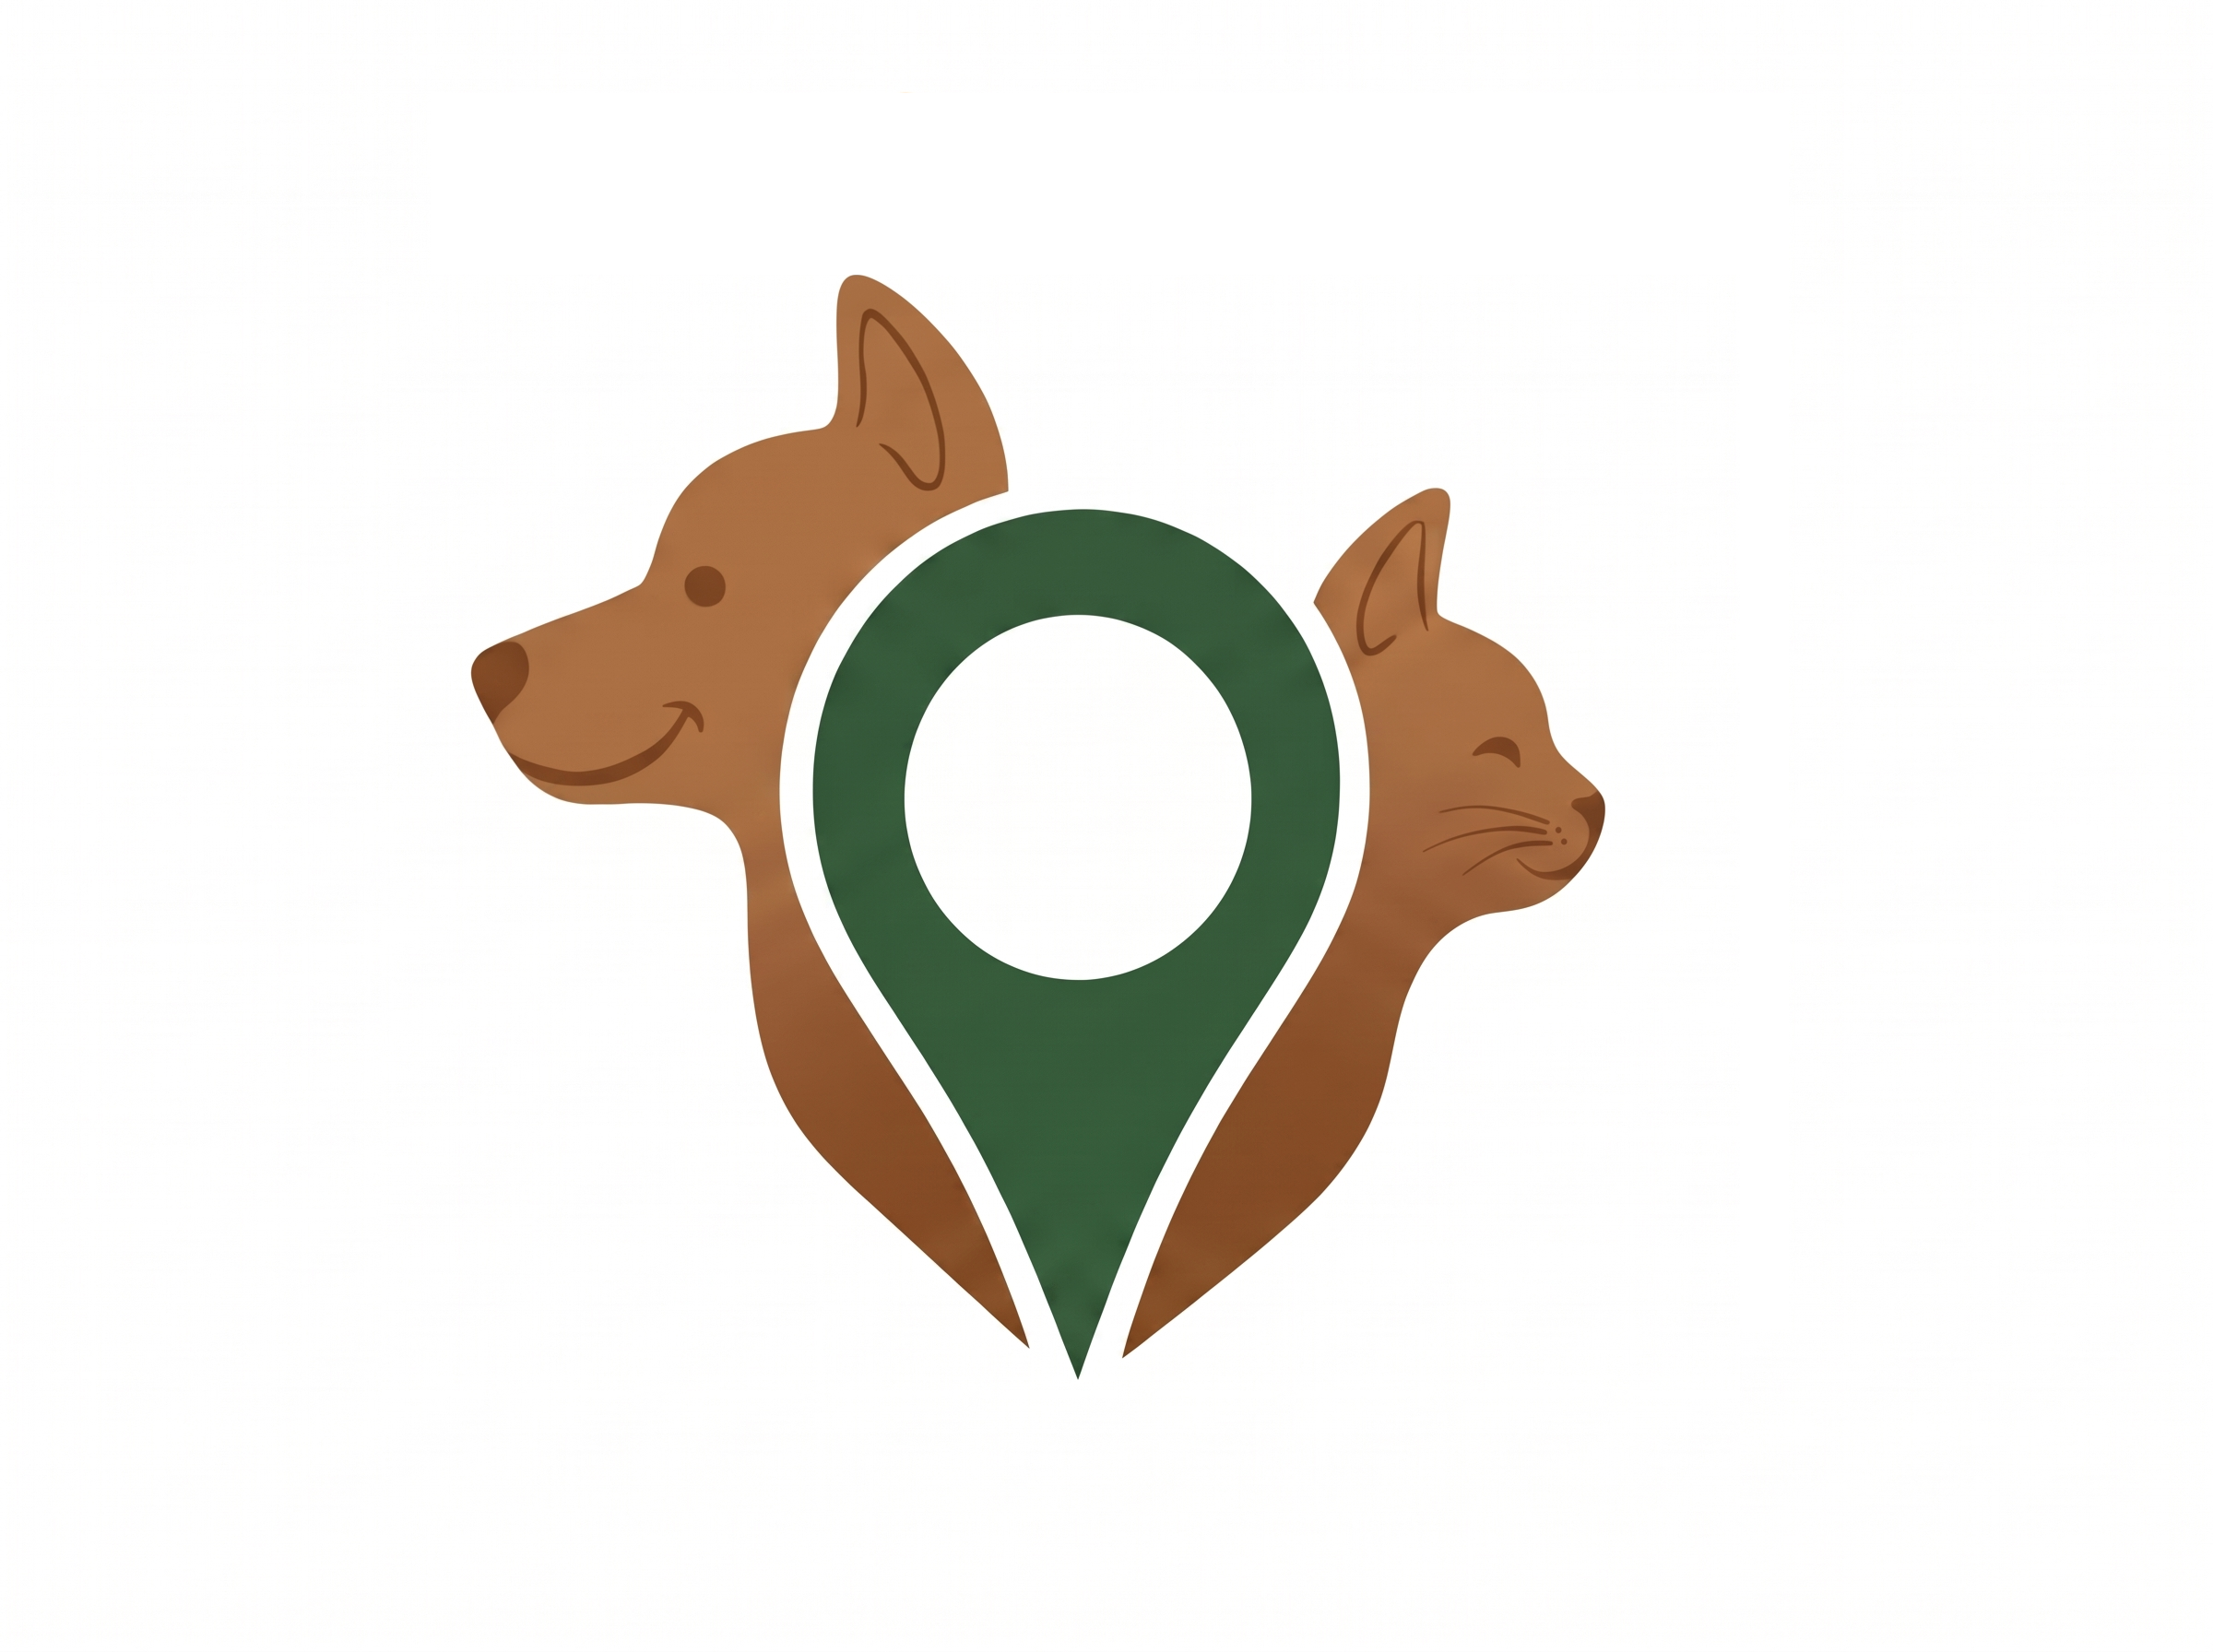
\includegraphics[width=0.42\textwidth]{imagens/03_arquitetura_design/figura13_logotipo_wefind.png}
    \fonte{Autoria própria (2026)}
\end{figure}

O símbolo gráfico reúne a silhueta de um cão à esquerda e de um gato à direita, circundando o marcador clássico de localização geográfica ao centro. Essa composição sintetiza a missão do sistema de atender às principais espécies domésticas, enquanto o marcador central enfatiza o recurso de geolocalização em mapa. As cores aplicadas reforçam a proposta: o tom Terracota acolhe as silhuetas dos animais e o Verde Esperança colore o pino de localização.

A leitura do símbolo comunica com clareza o propósito da ferramenta. A forma circular vazada no centro do marcador geográfico atua como uma lente de foco, sugerindo a atenção comunitária voltada para avistar, localizar e reencontrar o animal desaparecido.

O símbolo foi também preparado para atender às exigências técnicas dos sistemas móveis contemporâneos, como os ícones adaptativos do Android, que utilizam máscaras de corte circulares e quadradas com áreas de segurança bem definidas. O ícone também conta com versão monocromática para a barra de notificações do celular, facilitando o reconhecimento imediato de alertas e mensagens.

Na interface do aplicativo, a marca é utilizada de maneira consistente na tela de apresentação (\textit{splash screen}), nos cartazes digitais de busca gerados para impressão e nas carteirinhas com código QR vinculadas às coleiras. Essa padronização transmite seriedade e acolhimento, assegurando aos tutores e voluntários que a plataforma é um ambiente seguro e dedicado ao bem-estar animal.


\subsection{Paleta Cromática Oficial}

A definição cromática do WeFIND baseou-se nos princípios da psicologia das cores aplicados ao design digital (HELLER, 2021), buscando transmitir serenidade e afeto sem prejudicar a visibilidade de avisos urgentes. A Figura~\ref{fig:paleta_cores} apresenta a paleta oficial do sistema, organizada em três grupos estruturados.

\begin{figure}[H]
    \centering
    \caption{Identidade Visual e Paleta Cromática Oficial do WeFIND}
    \label{fig:paleta_cores}
    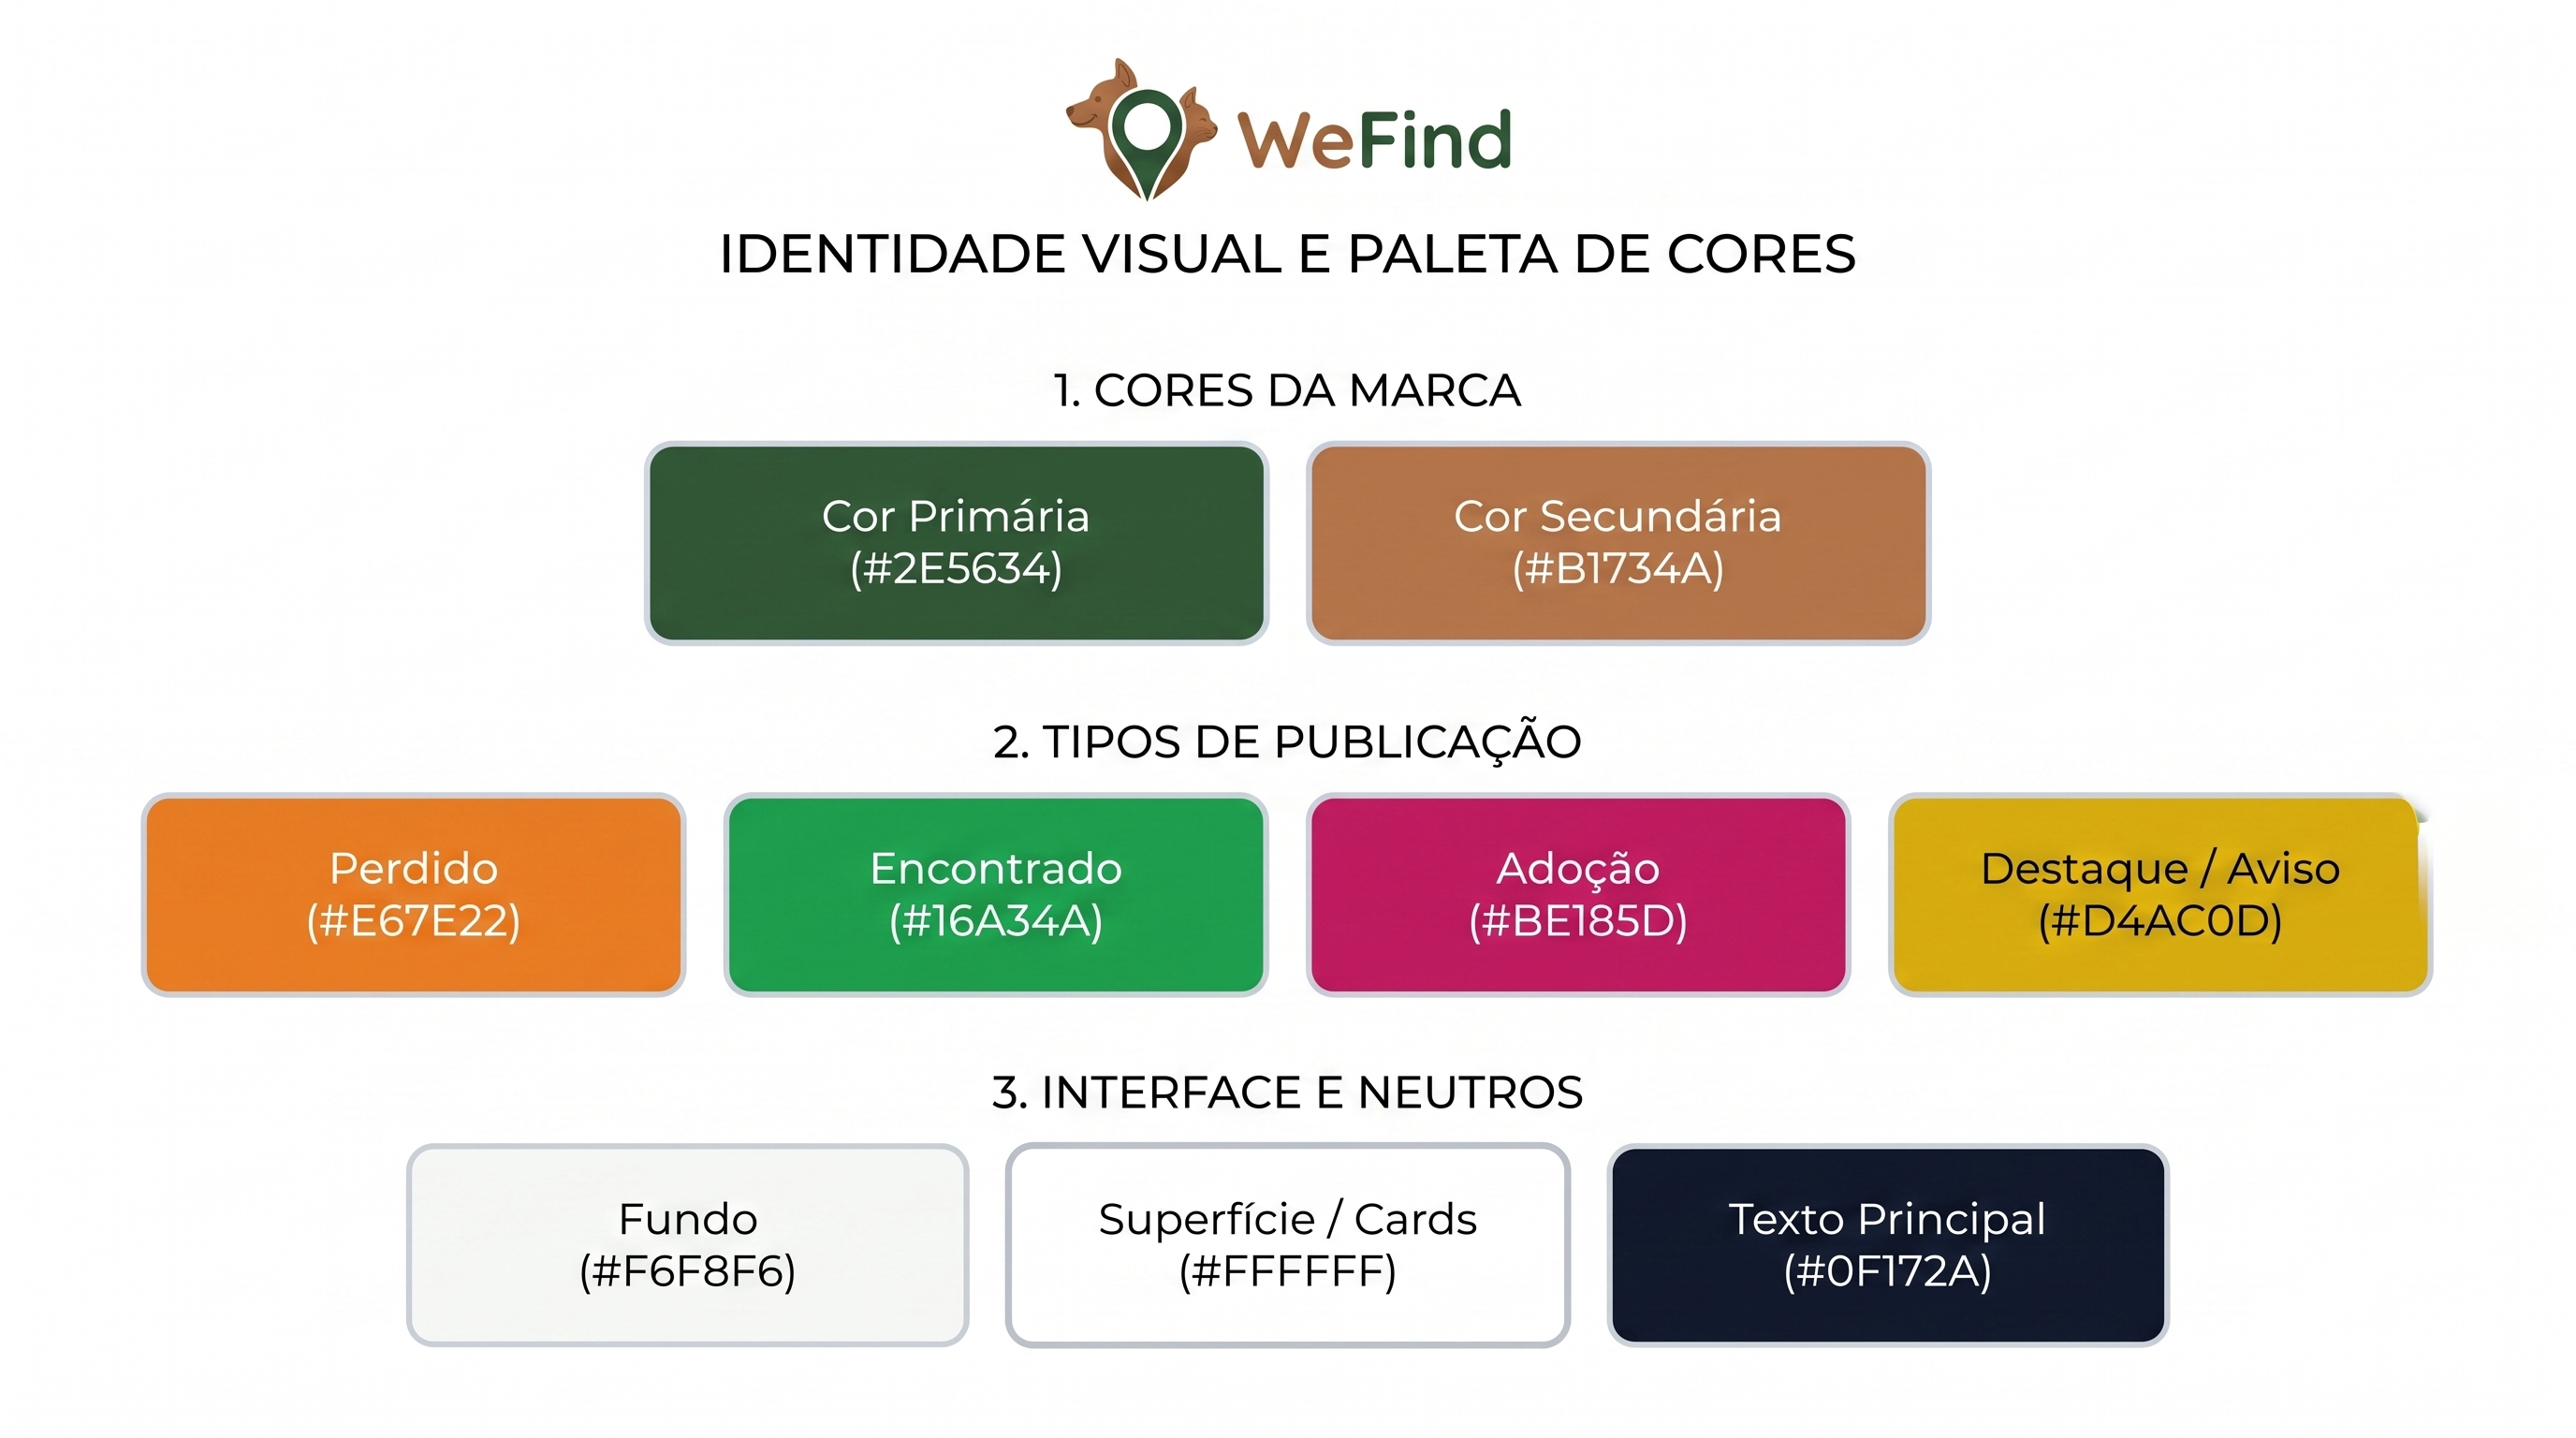
\includegraphics[height=5.2cm,keepaspectratio]{imagens/03_arquitetura_design/figura14_paleta_cores.jpeg}
    \par\vspace{0.15cm}
    {\footnotesize Figura~16.a) Cores da Plataforma \quad\textbar\quad Figura~16.b) Publicações \quad\textbar\quad Figura~16.c) Interface e Neutros\par}
    \fonte{Autoria própria (2026)}
\end{figure}

A organização das cores na Figura~\ref{fig:paleta_cores} estrutura-se em três blocos funcionais:

Na Figura~\ref{fig:paleta_cores}.a, apresentam-se as Cores da Plataforma. A Cor Primária em tom Verde (\#2E5634) evoca sentimentos de equilíbrio, esperança e solidez, sendo empregada como cor de fundo das barras superiores de navegação e em botões principais de ação. A Cor Secundária em tom Terracota (\#B1734A) remete ao cuidado, afeto e acolhimento animal, sendo utilizada em elementos secundários e detalhes de destaque.

Na Figura~\ref{fig:paleta_cores}.b, encontram-se as Cores Semânticas de Publicação, concebidas para permitir a triagem visual rápida do status de cada publicação: o tom Laranja Alerta (\#E67E22) sinaliza animais Perdidos; o Verde Sucesso (\#16A34A) identifica animais já Encontrados; o Magenta (\#BE185D) indica anúncios voltados à Adoção; e o tom Amarelo Dourado (\#D4AC0D) destaca Avisos urgentes e novos relatos de avistamento comunitário.

Na Figura~\ref{fig:paleta_cores}.c, reúnem-se as Cores de Interface e Elementos Neutros: a tonalidade cinza suave de Fundo (\#F6F8F6) evita fadiga ocular; o tom branco puro de Superfície (\#FFFFFF) destaca cartões e campos interativos; e a tipografia principal em tom Azul Noturno Escuro (\#0F172A) garante conformidade rigorosa com os níveis de contraste AA e AAA exigidos pelas diretrizes de acessibilidade WCAG.



\subsection{Funcionamento e Telas do Aplicativo}

O WeFIND organiza suas funcionalidades em fluxos diretos, orientados pela jornada do tutor e apoiados por uma barra de navegação inferior. As telas principais de acesso são apresentadas nas Figuras~\ref{fig:telas_autenticacao} e~\ref{fig:tela_cadastro_recuperacao}.

O fluxo de entrada foi planejado para atender tanto usuários que já possuem cadastro quanto pessoas que estão conhecendo a plataforma. A tela inicial concentra o acesso à conta e os recursos de recuperação, enquanto a apresentação do aplicativo oferece uma visão geral do serviço antes que o visitante decida realizar o cadastro.

\begin{figure}[H]
    \centering
    \caption{Telas de Login e Apresentação do Aplicativo WeFIND}
    \label{fig:telas_autenticacao}
    \vspace{0.15cm}
    \begin{minipage}[t]{0.48\textwidth}
        \centering
        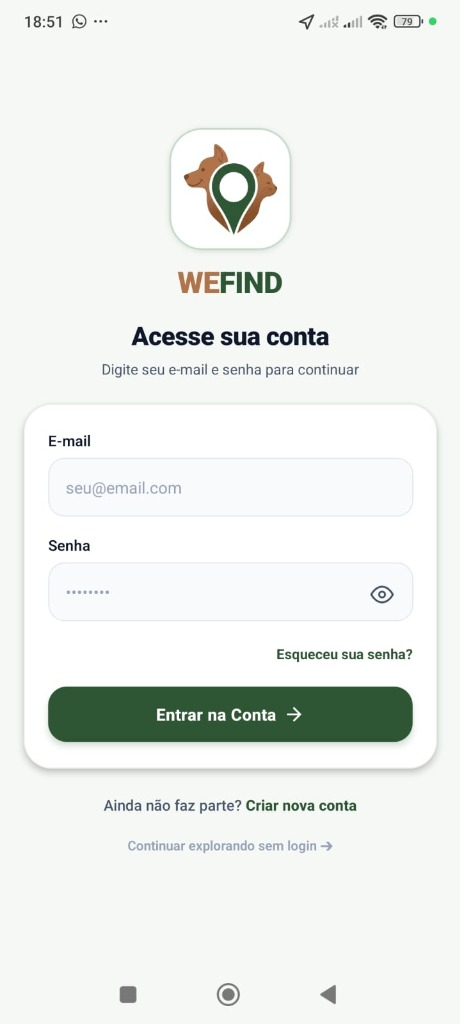
\includegraphics[height=11.6cm,keepaspectratio]{imagens/04_telas_aplicativo/tela-autenticacao-login.jpeg}
        \par\vspace{0.15cm}
        {\small Figura~\thefigure.a) Tela de Login}
    \end{minipage}
    \hfill
    \begin{minipage}[t]{0.48\textwidth}
        \centering
        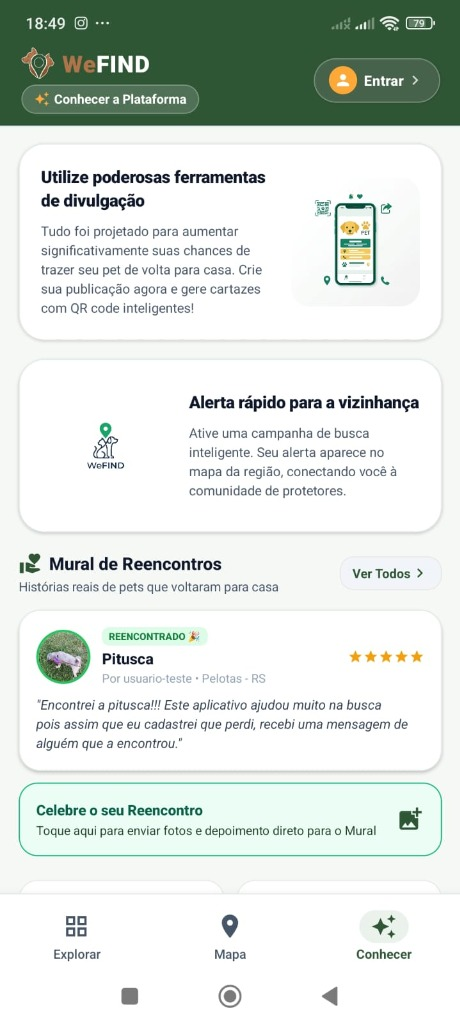
\includegraphics[height=11.6cm,keepaspectratio]{imagens/04_telas_aplicativo/tela-apresentacao-conhecer.jpeg}
        \par\vspace{0.15cm}
        {\small Figura~\thefigure.b) Apresentação do Aplicativo}
    \end{minipage}
    \par\vspace{0.15cm}
    \fonte{Autoria própria (2026)}
\end{figure}

A tela de login reúne os campos de e-mail e senha, a recuperação de credenciais e a possibilidade de conhecer o aplicativo antes do cadastro. A Figura~\ref{fig:telas_autenticacao}.b apresenta essa opção de apresentação, que permite ao visitante compreender a finalidade do WeFIND e consultar suas principais funções antes de criar uma conta. Assim, as duas telas formam um fluxo inicial simples: o usuário pode entrar com uma conta existente ou conhecer a proposta do aplicativo antes de prosseguir para o cadastro. Essa organização reduz o número de decisões iniciais e orienta o usuário para as ações essenciais.

Quando o visitante decide continuar, o fluxo conduz ao cadastro ou à recuperação da conta, conforme sua situação. A Figura~\ref{fig:tela_cadastro_recuperacao} apresenta essas duas alternativas de acesso e mostra como o aplicativo mantém os procedimentos concentrados em telas simples.

\begin{figure}[H]
    \centering
    \caption{Cadastro de Usuário e Recuperação de Conta}
    \label{fig:tela_cadastro_recuperacao}
    \vspace{0.15cm}
    \begin{minipage}[t]{0.48\textwidth}
        \centering
        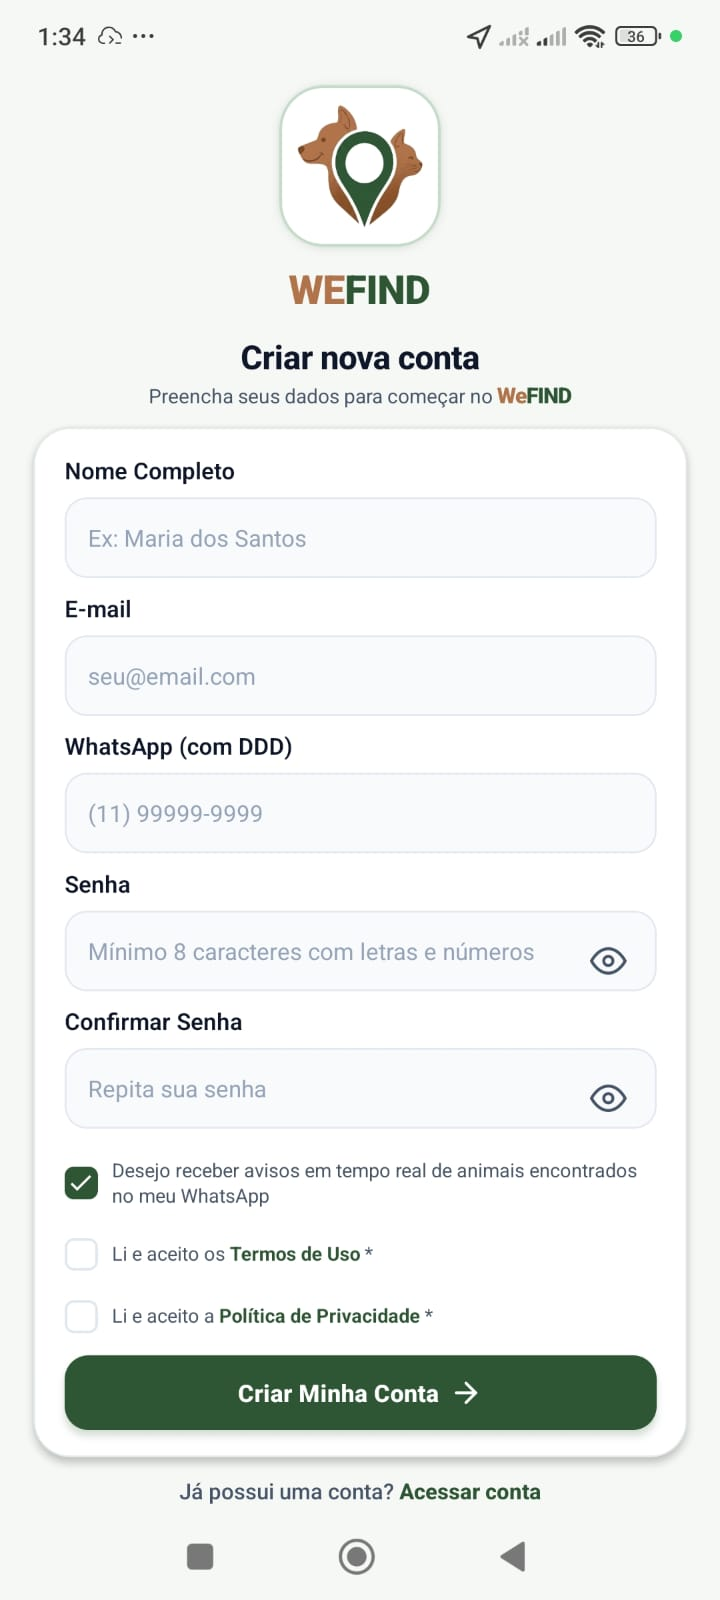
\includegraphics[height=11.6cm,keepaspectratio]{imagens/04_telas_aplicativo/tela-criar-conta.jpeg}
        \par\vspace{0.15cm}
        {\small Figura~\thefigure.a) Cadastro de Usuário}
    \end{minipage}
    \hfill
    \begin{minipage}[t]{0.48\textwidth}
        \centering
        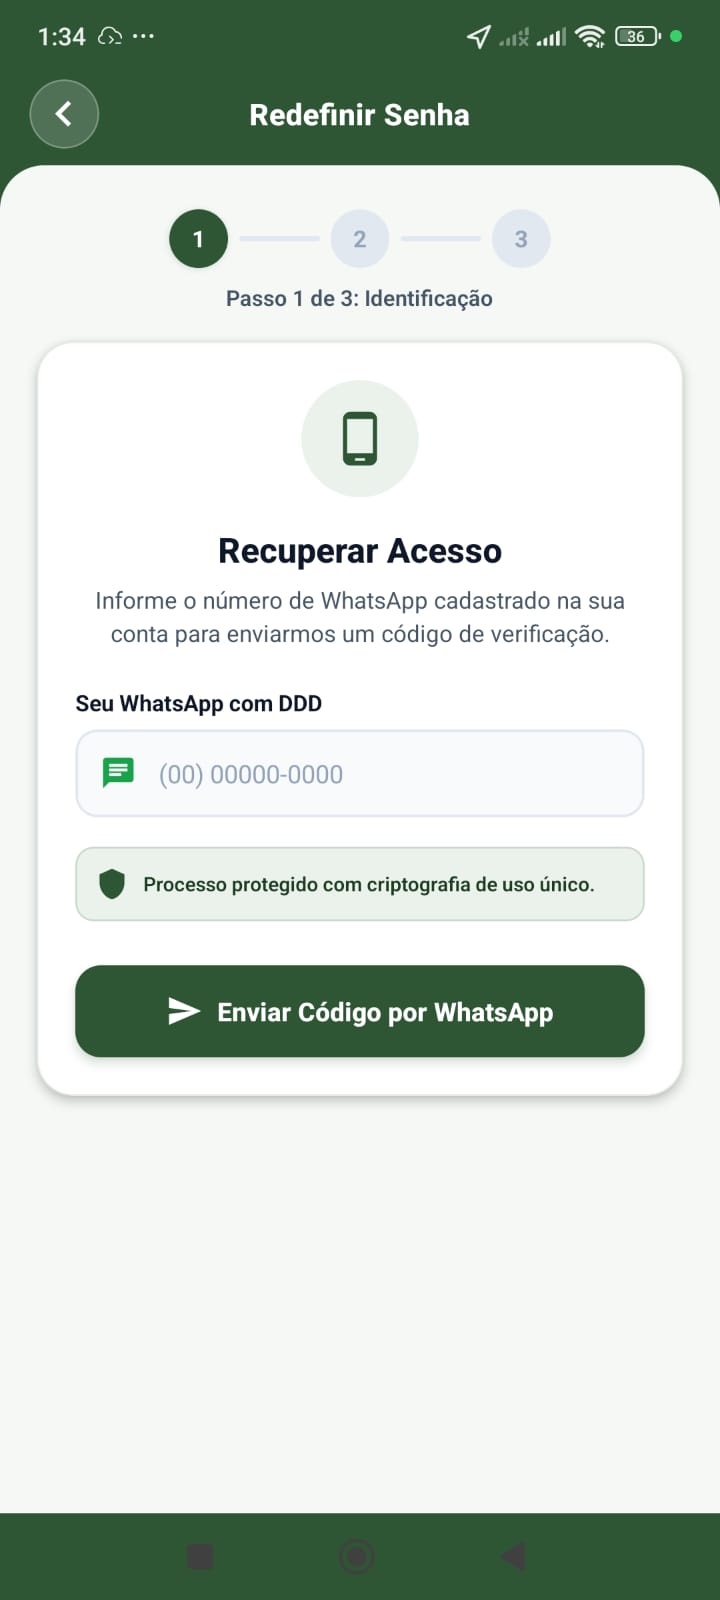
\includegraphics[height=11.6cm,keepaspectratio]{imagens/04_telas_aplicativo/tela-recuperar-senha.jpeg}
        \par\vspace{0.15cm}
        {\small Figura~\thefigure.b) Recuperação de Senha}
    \end{minipage}
    \par\vspace{0.12cm}
    \fonte{Autoria própria (2026)}
\end{figure}

O cadastro solicita os dados necessários para a identificação do participante, enquanto a recuperação de conta oferece um caminho específico para redefinir a senha. Os dois fluxos mantêm mensagens objetivas e campos compatíveis com o uso em dispositivos móveis.

Na Figura~\ref{fig:tela_cadastro_recuperacao}.a, o usuário informa os dados necessários para criar o perfil. Na Figura~\ref{fig:tela_cadastro_recuperacao}.b, solicita a recuperação da senha para restabelecer o acesso. A separação evita misturar o cadastro inicial com uma situação de manutenção da conta.

Mesmo sem autenticação imediata, o modo visitante permite consultar publicações e localizar informações básicas de animais perdidos ou encontrados. Para preservar a segurança das interações, ações como publicar, comentar ou enviar mensagens dependem de autenticação; essa alternativa de consulta não exige uma figura própria.

A localização é um recurso central do sistema, pois permite relacionar publicações, avistamentos e distâncias. Antes de exibir os resultados, o aplicativo solicita a permissão necessária e, em seguida, oferece recursos para consultar os pontos registrados. A Figura~\ref{fig:tela_mapa} reúne essas etapas, incluindo a consulta de rota.

\begin{figure}[H]
    \centering
    \caption{Mapa Interativo, Marcadores e Rota até o Animal}
    \label{fig:tela_mapa}
    \vspace{0.15cm}
    \begin{minipage}[t]{0.31\textwidth}
        \centering
        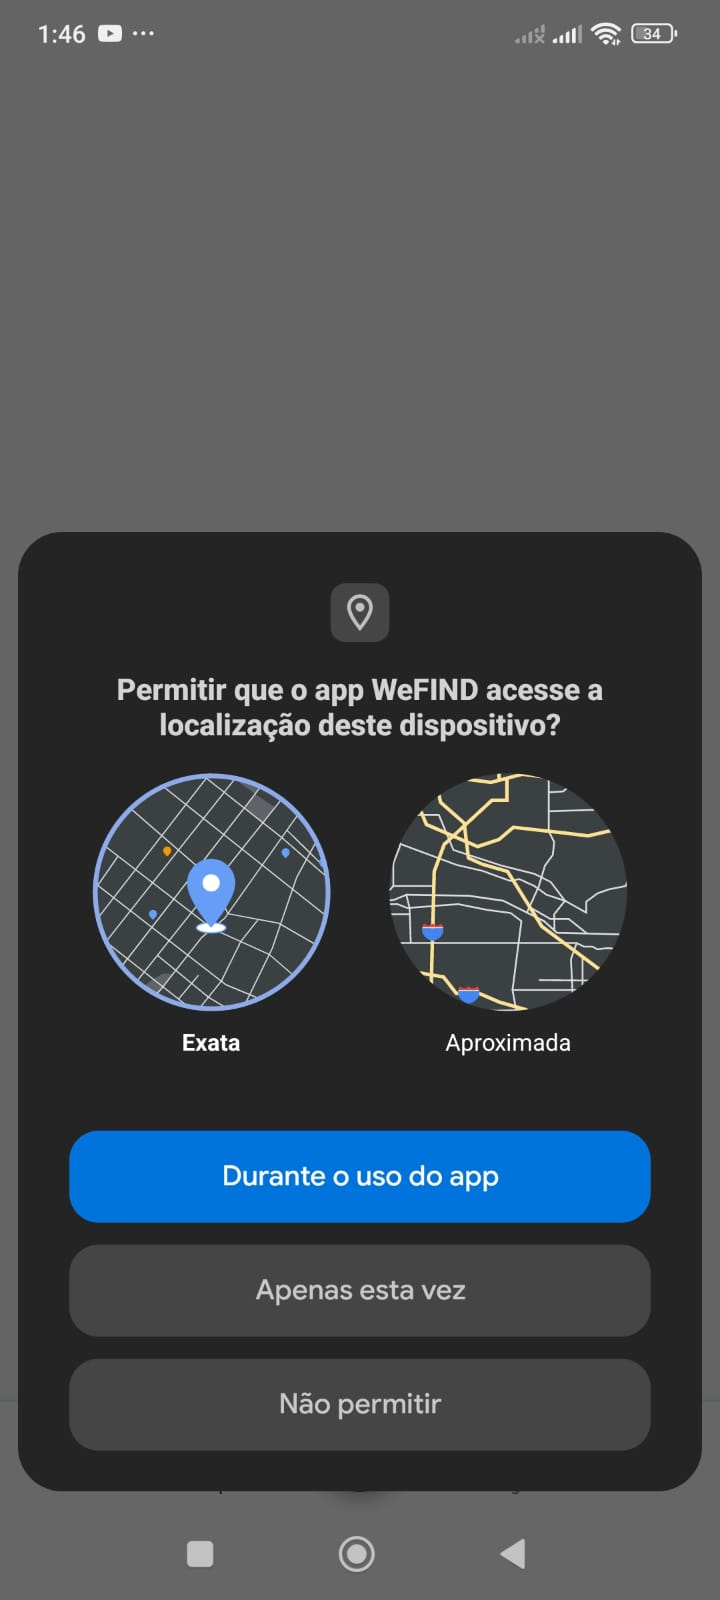
\includegraphics[height=9.2cm,keepaspectratio]{imagens/04_telas_aplicativo/tela-permissao-localizacao.jpeg}
        \par\vspace{0.12cm}
        {\small Figura~\thefigure.a) Permissão de Localização}
    \end{minipage}
    \hfill
    \begin{minipage}[t]{0.31\textwidth}
        \centering
        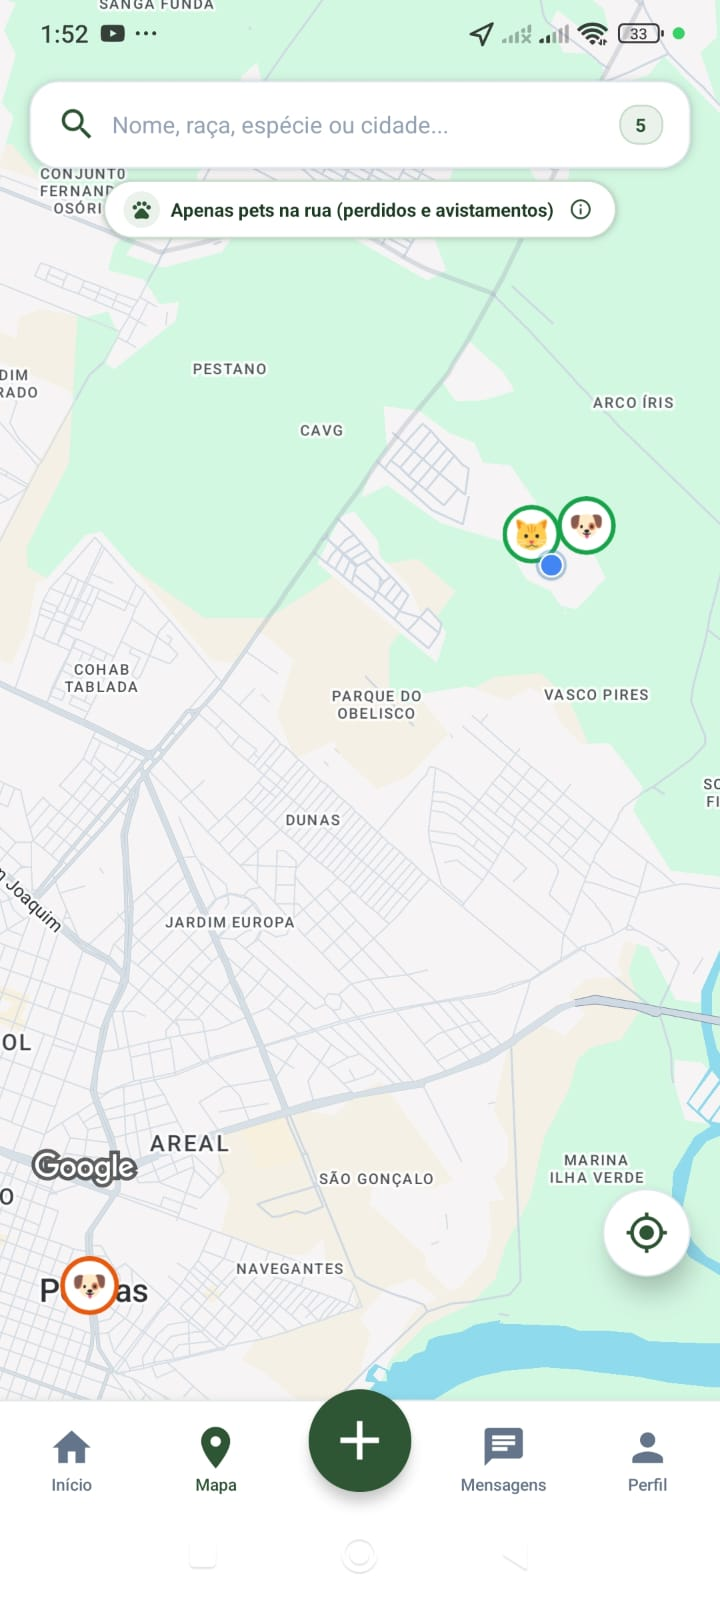
\includegraphics[height=9.2cm,keepaspectratio]{imagens/04_telas_aplicativo/tela-mapa-principal.jpeg}
        \par\vspace{0.12cm}
        {\small Figura~\thefigure.b) Mapa Interativo}
    \end{minipage}
    \hfill
    \begin{minipage}[t]{0.31\textwidth}
        \centering
        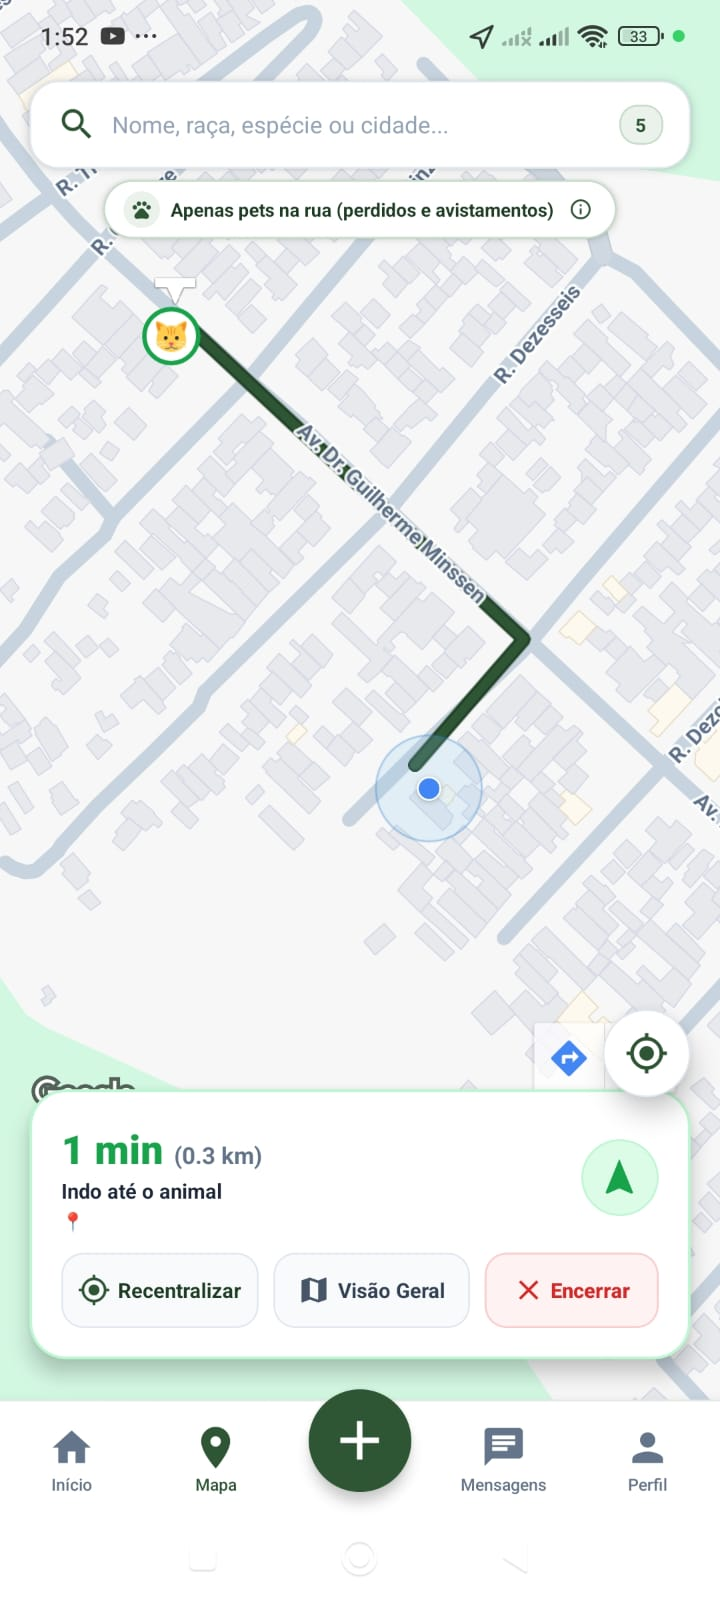
\includegraphics[height=9.2cm,keepaspectratio]{imagens/04_telas_aplicativo/tela-mapa-rota-animal.jpeg}
        \par\vspace{0.12cm}
        {\small Figura~\thefigure.c) Rota até o Animal}
    \end{minipage}
    \par\vspace{0.12cm}
    \fonte{Autoria própria (2026)}
\end{figure}

A Figura~\ref{fig:tela_mapa}.a mostra a solicitação de acesso à localização. A Figura~\ref{fig:tela_mapa}.b apresenta o mapa com os marcadores das publicações, enquanto a Figura~\ref{fig:tela_mapa}.c demonstra a rota até o animal selecionado. Esses elementos apoiam a busca sem substituir a avaliação do usuário sobre as condições do local.

O formulário unificado de registro contempla as situações mais frequentes da plataforma: o tutor que perdeu o animal, a pessoa que encontrou um animal e o cidadão que apenas realizou um avistamento. A separação inicial das modalidades ajuda o usuário a escolher o caminho correspondente ao seu caso. A Figura~\ref{fig:tela_registro_perdi_encontrei} apresenta esses caminhos principais.

\begin{figure}[H]
    \centering
    \caption{Registro de Animal: Perdi, Encontrei e Avistamento}
    \label{fig:tela_registro_perdi_encontrei}
    \vspace{0.15cm}
    \begin{minipage}[t]{0.31\textwidth}
        \centering
        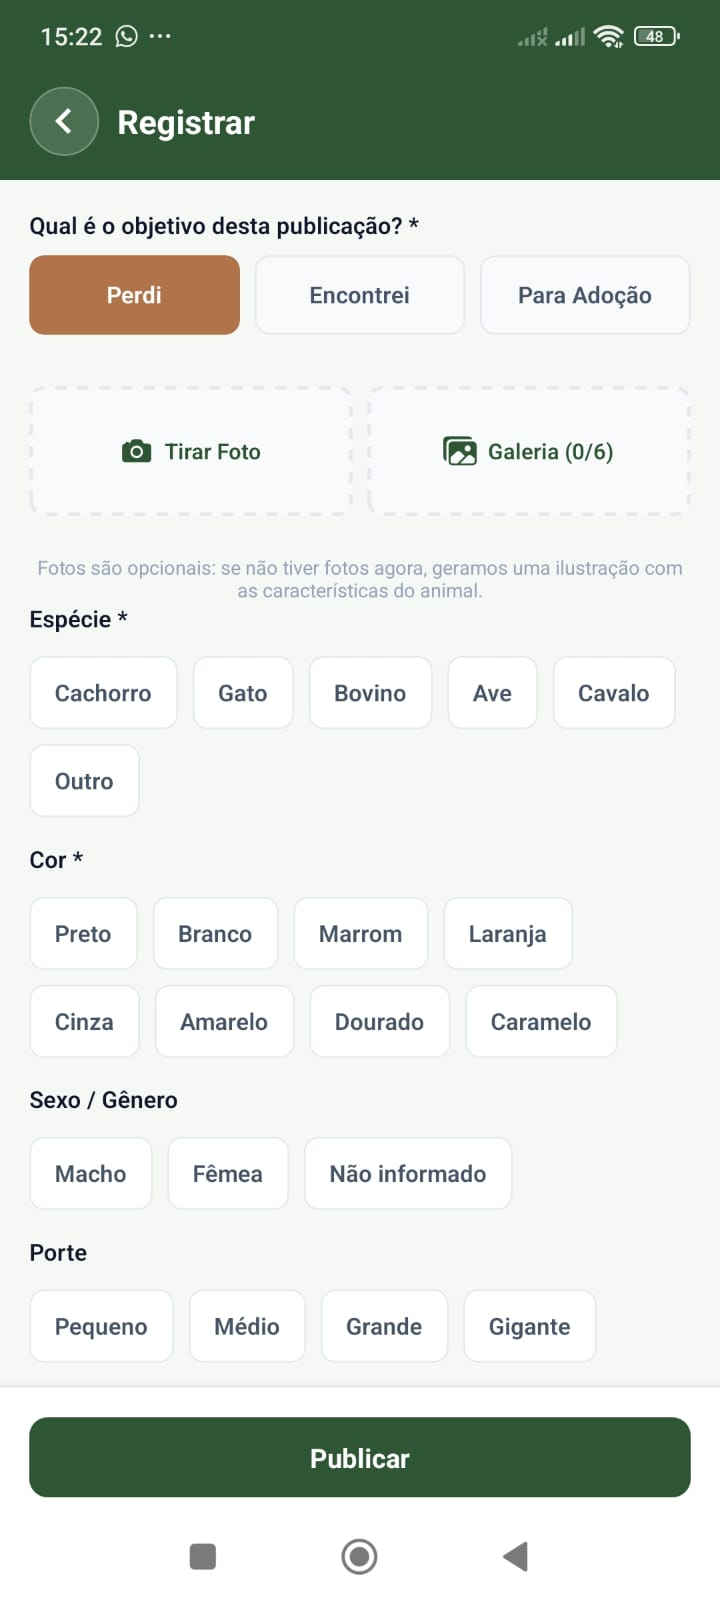
\includegraphics[height=9.2cm,keepaspectratio]{imagens/04_telas_aplicativo/tela-registro-perdi.jpeg}
        \par\vspace{0.12cm}
        {\small Figura~\thefigure.a) Perdi um Animal}
    \end{minipage}
    \hfill
    \begin{minipage}[t]{0.31\textwidth}
        \centering
        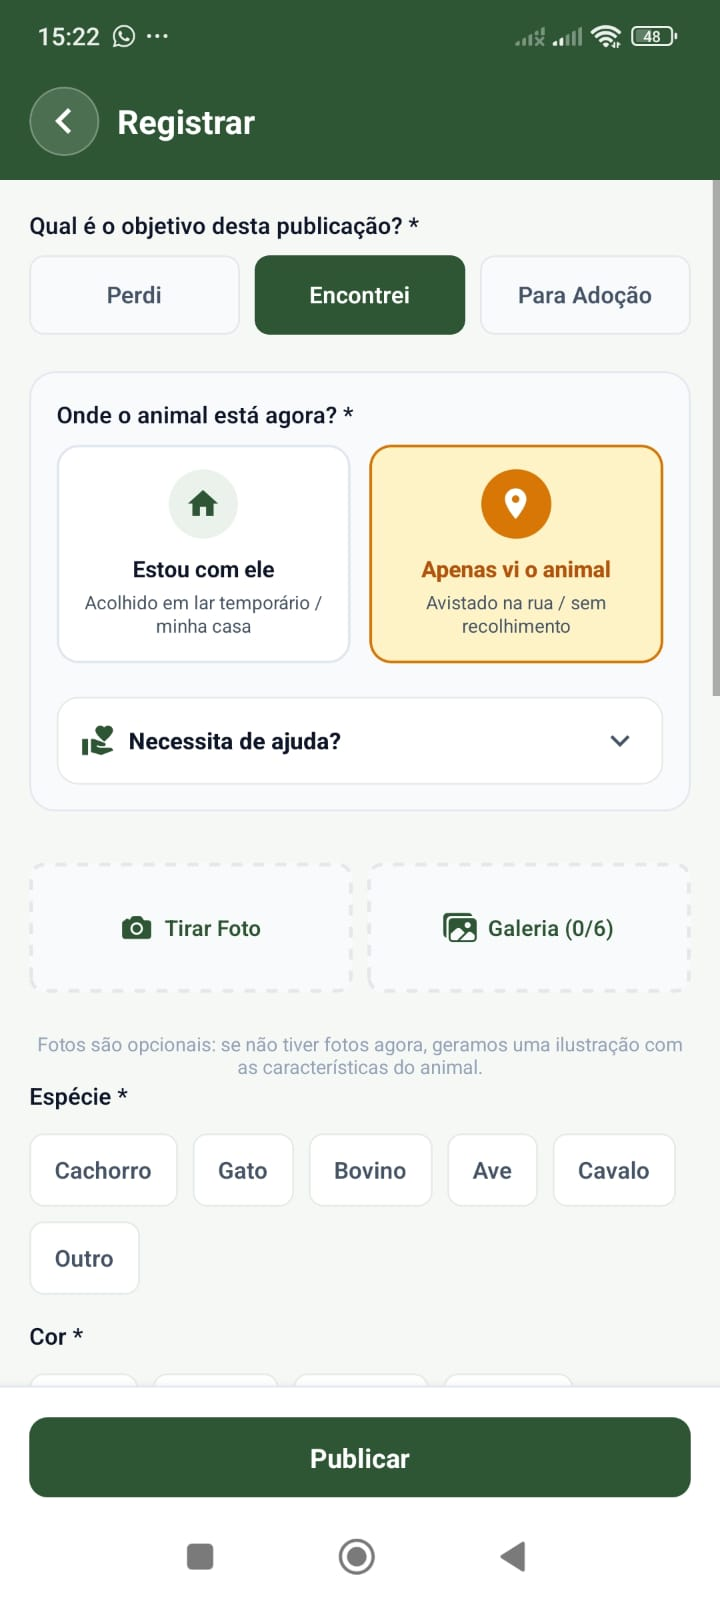
\includegraphics[height=9.2cm,keepaspectratio]{imagens/04_telas_aplicativo/tela-registro-encontrei-avistamento.jpeg}
        \par\vspace{0.12cm}
        {\small Figura~\thefigure.b) Encontrei um Animal}
    \end{minipage}
    \hfill
    \begin{minipage}[t]{0.31\textwidth}
        \centering
        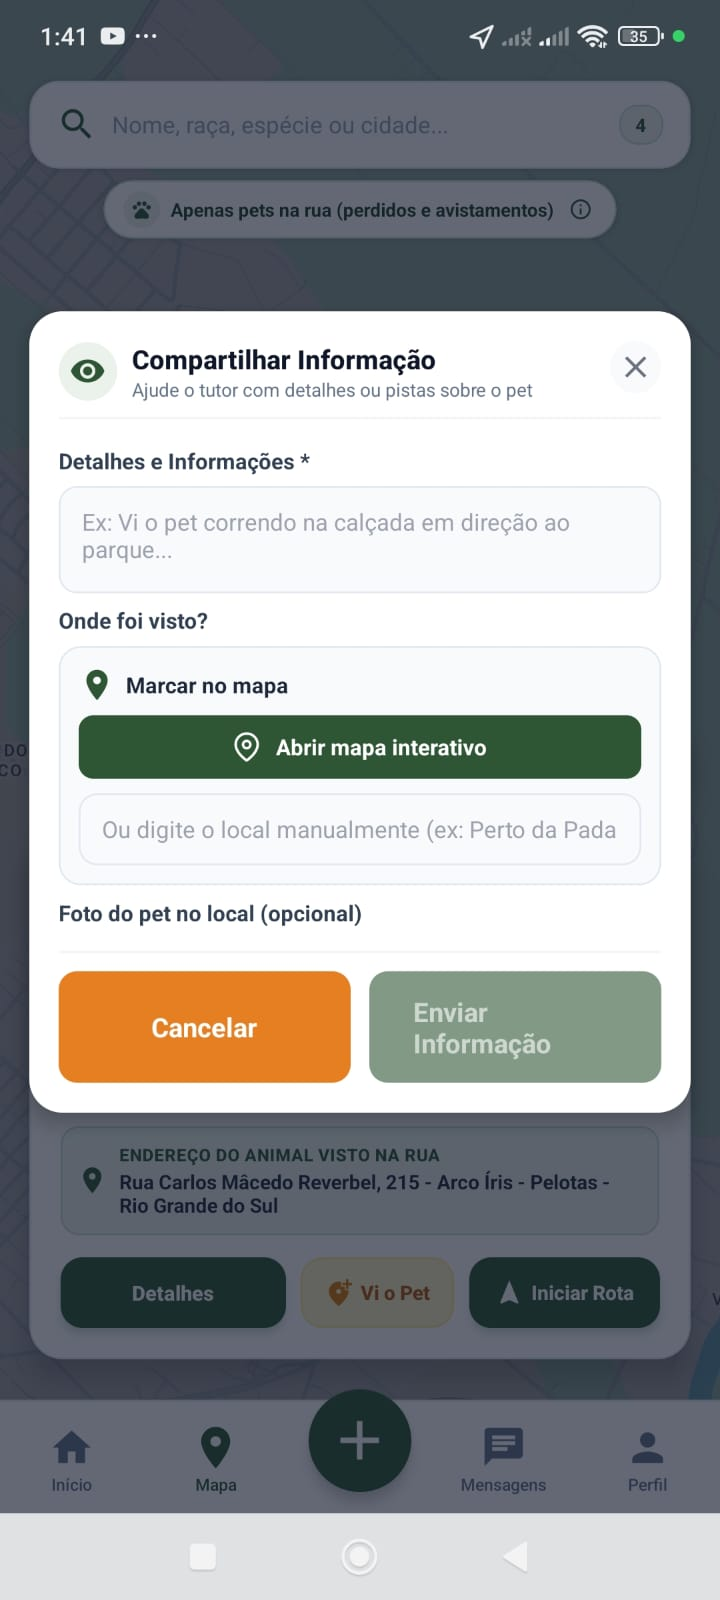
\includegraphics[height=9.2cm,keepaspectratio]{imagens/04_telas_aplicativo/tela-registro-avistamento.jpeg}
        \par\vspace{0.12cm}
        {\small Figura~\thefigure.c) Registrei um Avistamento}
    \end{minipage}
    \par\vspace{0.12cm}
    \fonte{Autoria própria (2026)}
\end{figure}

A Figura~\ref{fig:tela_registro_perdi_encontrei}.a representa o registro de um animal perdido, com foco nas características necessárias à busca. A Figura~\ref{fig:tela_registro_perdi_encontrei}.b corresponde ao cadastro de um animal encontrado, enquanto a Figura~\ref{fig:tela_registro_perdi_encontrei}.c registra um avistamento vinculado a uma localização. A escolha da modalidade define os campos exibidos e reduz ambiguidades no envio das informações.

A ficha de cada publicação concentra as informações necessárias para consulta e acompanhamento do caso. Além da visualização dos dados do animal, o sistema apresenta ações diferentes conforme a publicação pertença ou não ao usuário. Essa distinção é ilustrada na Figura~\ref{fig:tela_detalhes}.

\begin{figure}[H]
    \centering
    \caption{Detalhes da Publicação e Painel de Gestão do Autor}
    \label{fig:tela_detalhes}
    \vspace{0.15cm}
    \begin{minipage}[t]{0.48\textwidth}
        \centering
        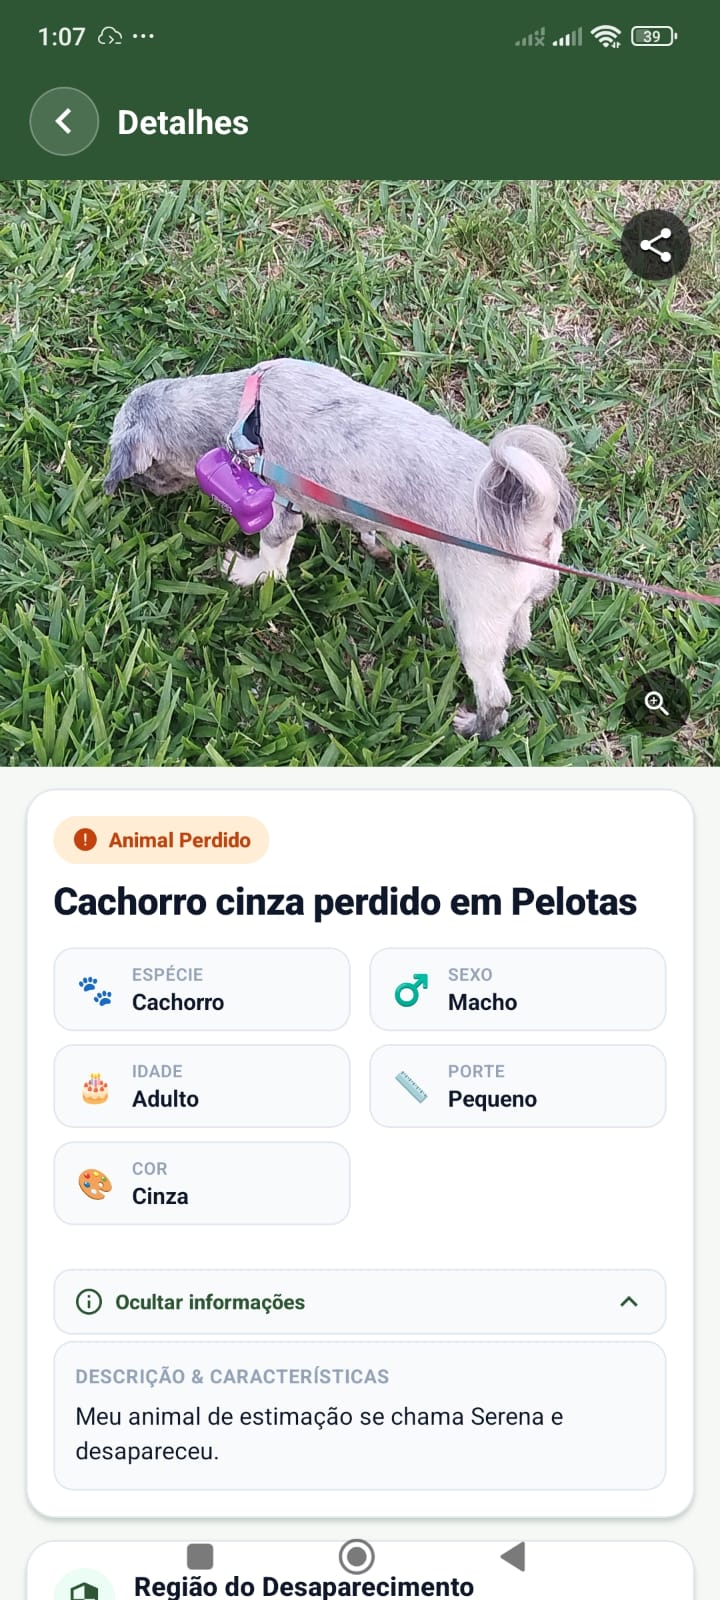
\includegraphics[height=10.8cm,keepaspectratio]{imagens/04_telas_aplicativo/tela-detalhes-do-animal.jpeg}
        \par\vspace{0.15cm}
        {\small Figura~\thefigure.a) Visualização Pública}
    \end{minipage}
    \hfill
    \begin{minipage}[t]{0.48\textwidth}
        \centering
        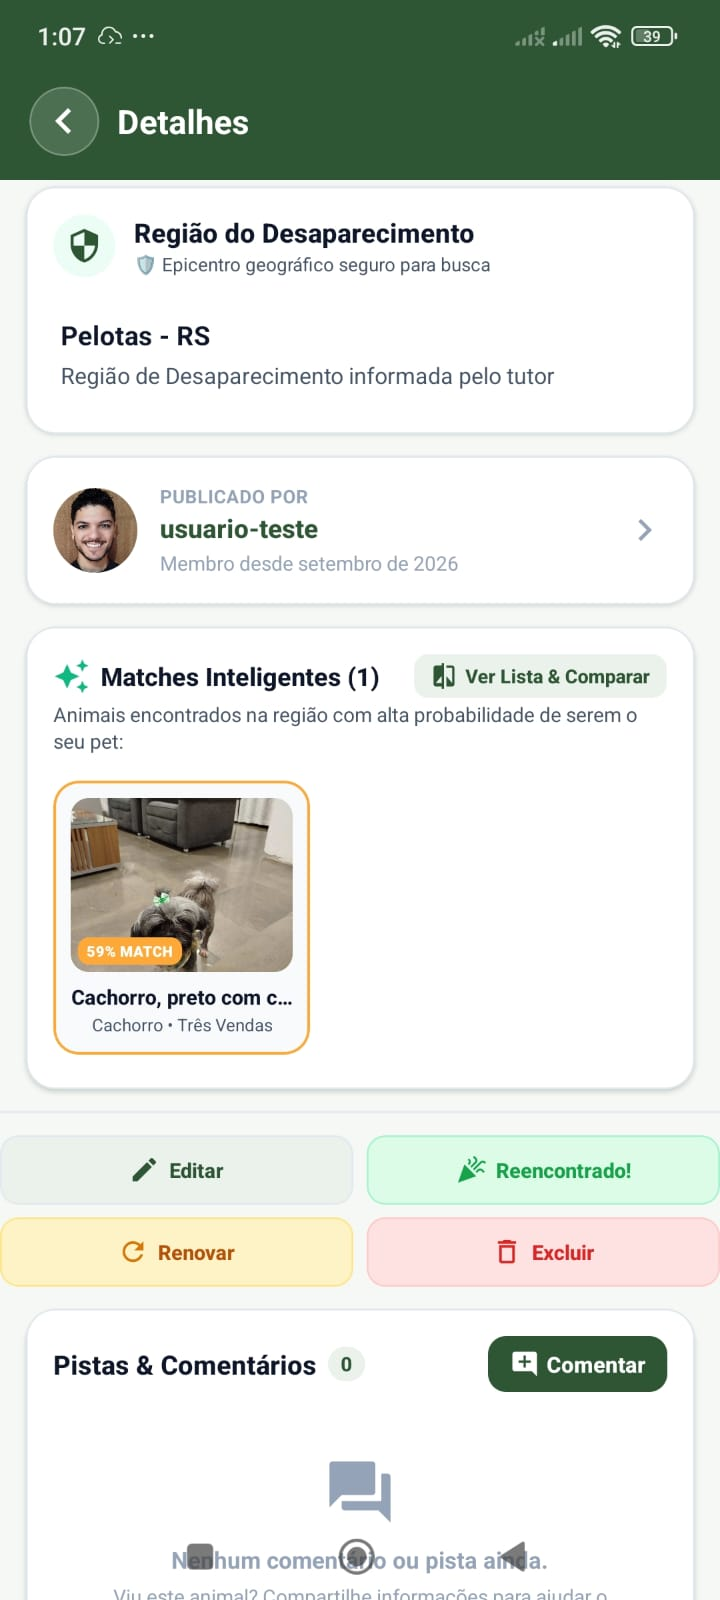
\includegraphics[height=10.8cm,keepaspectratio]{imagens/04_telas_aplicativo/tela-detalhes-do-animal-minha-publicacao-botoes-renovacao-publicacao-editar-excluir-marcar-reencontro.jpeg}
        \par\vspace{0.15cm}
        {\small Figura~\thefigure.b) Gestão do Autor}
    \end{minipage}
    \par\vspace{0.12cm}
    \fonte{Autoria própria (2026)}
\end{figure}

A Figura~\ref{fig:tela_detalhes}.a exibe a visualização pública, com fotografias, características físicas, localização aproximada e meios de envio de pistas. A Figura~\ref{fig:tela_detalhes}.b mostra a área de gestão do autor, que oferece ações de edição, renovação e encerramento do caso. Dessa forma, são mantidos distintos os níveis de acesso.

O sistema também cruza atributos de publicações para apresentar correspondências potenciais. Esse recurso foi organizado em duas etapas: primeiro, a listagem dos candidatos e, depois, a consulta detalhada dos atributos considerados. A Figura~\ref{fig:tela_correspondencias} mostra esse fluxo.

\begin{figure}[H]
    \centering
    \caption{Correspondências entre Publicações e Similaridade de Atributos}
    \label{fig:tela_correspondencias}
    \vspace{0.15cm}
    \begin{minipage}[t]{0.48\textwidth}
        \centering
        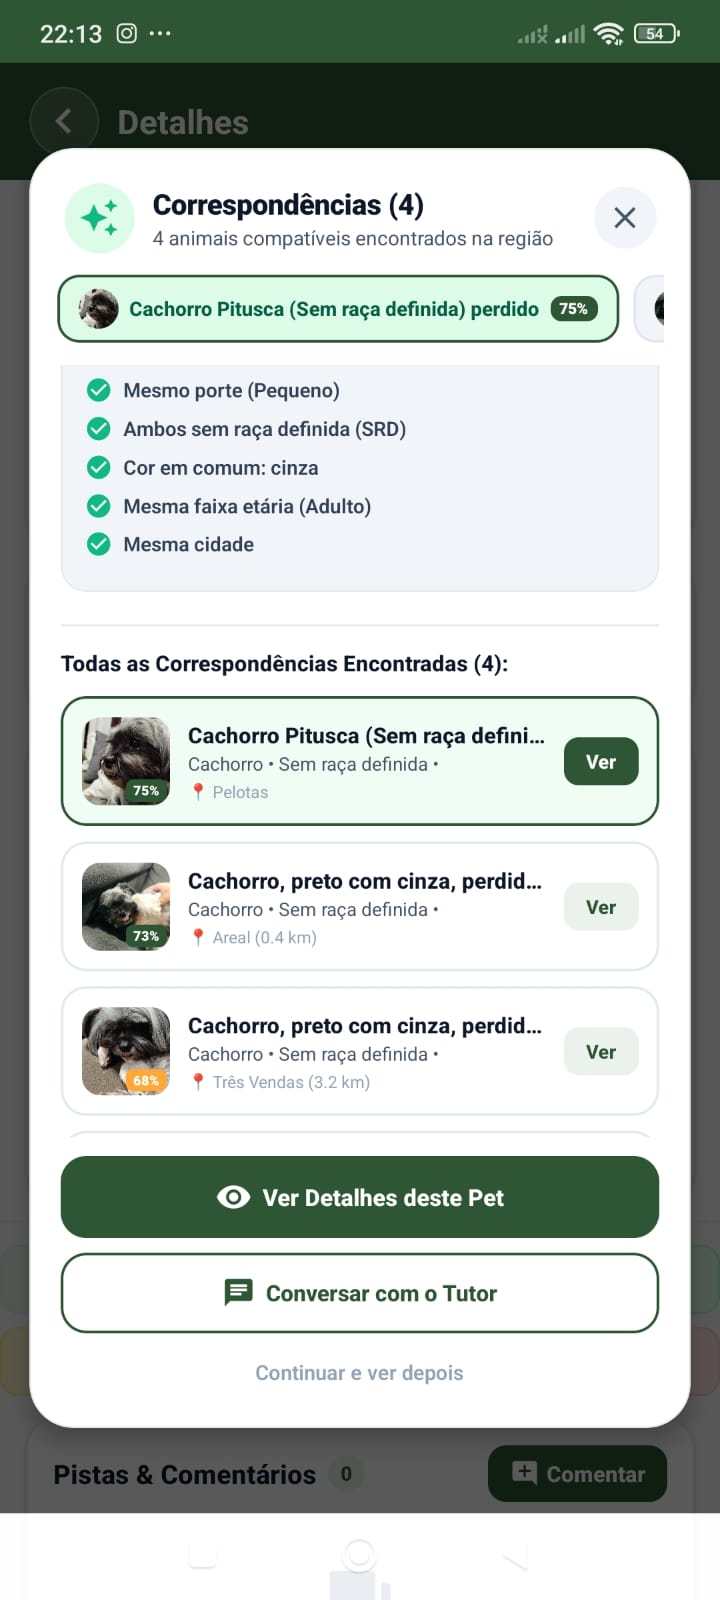
\includegraphics[height=10.8cm,keepaspectratio]{imagens/04_telas_aplicativo/tela-correspondencias2.jpeg}
        \par\vspace{0.15cm}
        {\small Figura~\thefigure.a) Lista de Correspondências}
    \end{minipage}
    \hfill
    \begin{minipage}[t]{0.48\textwidth}
        \centering
        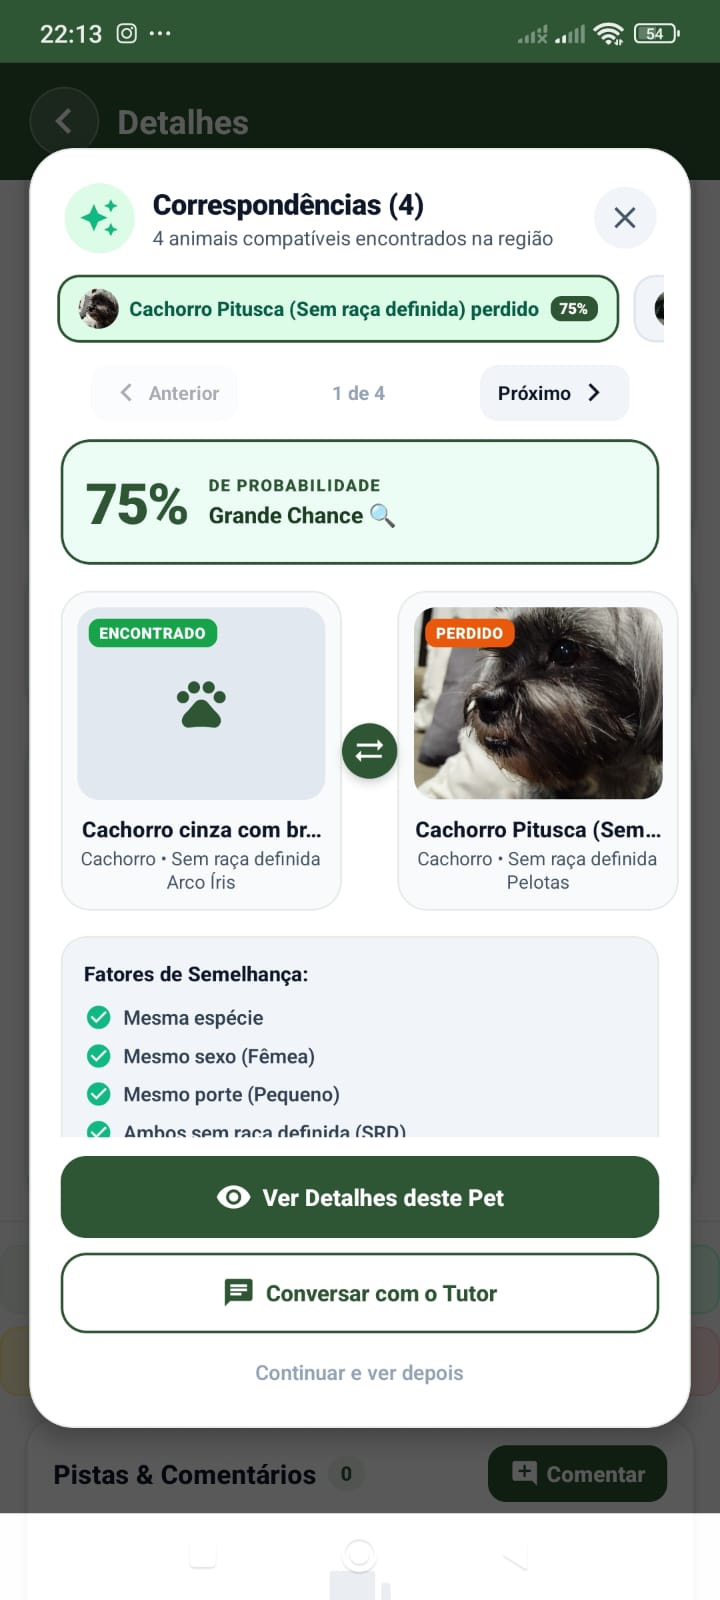
\includegraphics[height=10.8cm,keepaspectratio]{imagens/04_telas_aplicativo/tela-correspondencias.jpeg}
        \par\vspace{0.15cm}
        {\small Figura~\thefigure.b) Comparação de Atributos}
    \end{minipage}
    \par\vspace{0.12cm}
    \fonte{Autoria própria (2026)}
\end{figure}

A Figura~\ref{fig:tela_correspondencias}.a apresenta a lista de correspondências ordenada por similaridade e distância. A Figura~\ref{fig:tela_correspondencias}.b mostra a comparação dos atributos entre os registros selecionados. O resultado serve como apoio à decisão e não substitui a confirmação humana da identidade do animal.

Por fim, os animais cadastrados pelo usuário podem ser consultados em um painel próprio e em uma carteirinha digital. Esse recurso concentra informações preventivas que podem ser acessadas mesmo quando ainda não existe uma publicação de animal perdido. A Figura~\ref{fig:tela_meus_pets_rg} apresenta essas duas telas.

\begin{figure}[H]
    \centering
    \caption{Carteirinha Digital e Gestão dos Pets Tutelados}
    \label{fig:tela_meus_pets_rg}
    \vspace{0.15cm}
    \begin{minipage}[t]{0.48\textwidth}
        \centering
        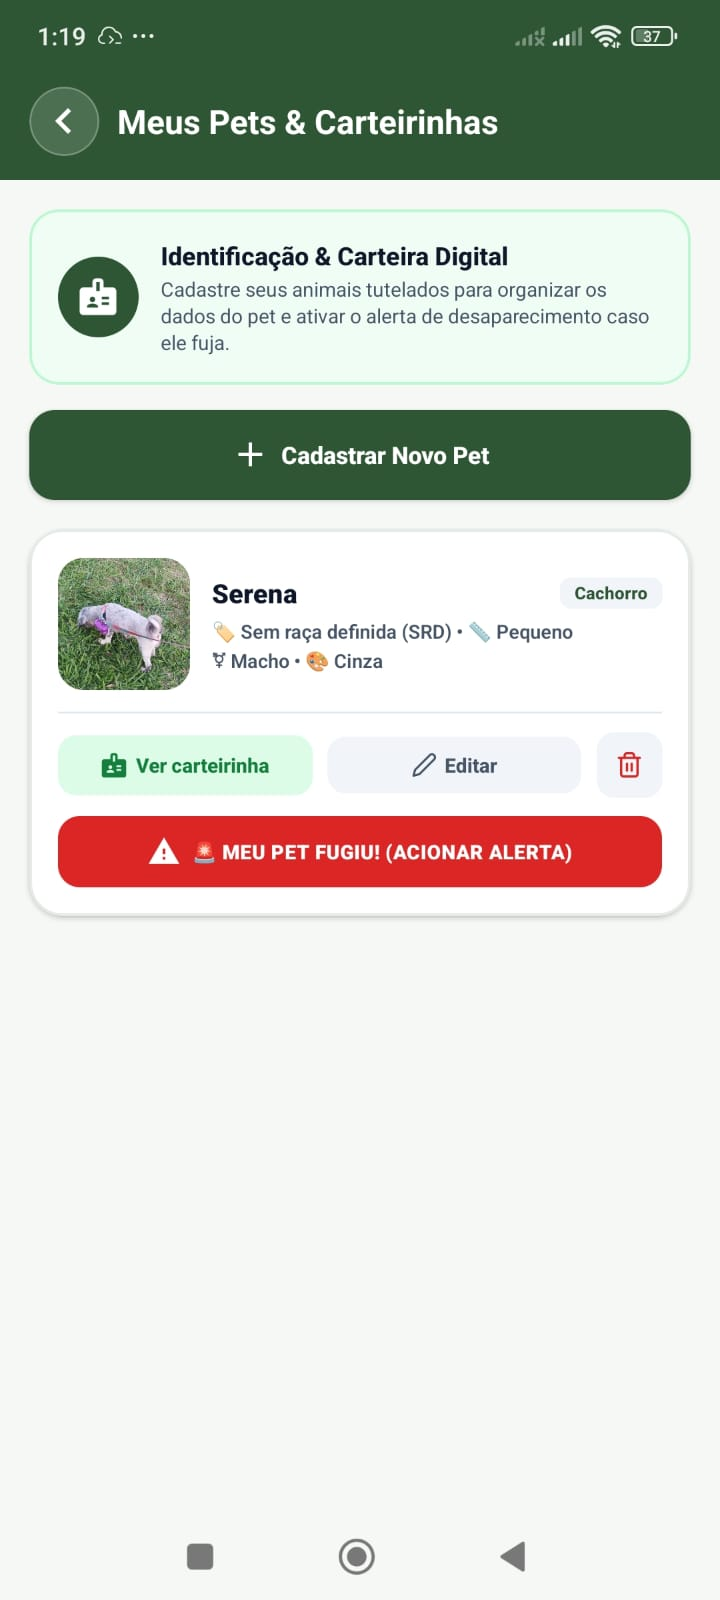
\includegraphics[height=10.8cm,keepaspectratio]{imagens/04_telas_aplicativo/tela-meus-pets-carteirinha-digital.jpeg}
        \par\vspace{0.15cm}
        {\small Figura~\thefigure.a) Painel de Pets}
    \end{minipage}
    \hfill
    \begin{minipage}[t]{0.48\textwidth}
        \centering
        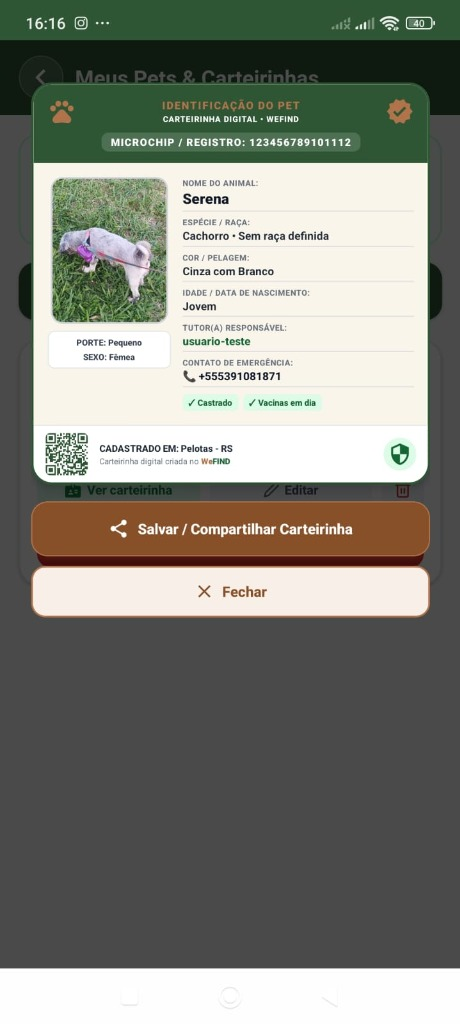
\includegraphics[height=10.8cm,keepaspectratio]{imagens/04_telas_aplicativo/tela-carteirinha-digital-rg.jpeg}
        \par\vspace{0.15cm}
        {\small Figura~\thefigure.b) Carteirinha com Código QR}
    \end{minipage}
    \par\vspace{0.12cm}
    \fonte{Autoria própria (2026)}
\end{figure}

A Figura~\ref{fig:tela_meus_pets_rg}.a mostra o painel de pets cadastrados e o acesso aos respectivos dados. A Figura~\ref{fig:tela_meus_pets_rg}.b apresenta a carteirinha digital com os dados essenciais e o código QR para facilitar a identificação. O recurso fortalece a prevenção sem duplicar o cadastro de uma publicação.
